% CS 418: Intro to Data Science — Worksheet 20 (20-week10-day2)
% Week 10, Wednesday 2026-10-28
% Compile with: latexmk -pdf worksheet.tex

\documentclass[11pt]{article}

% ── Packages ──────────────────────────────────────────────────────────────────
% The wide right margin is the open-ended notes column, half of the 7.2in between the outer margins less a 0.3in gutter; the header and title block span both.
\usepackage[margin=0.65in, right=4.4in, headheight=14pt]{geometry}
\usepackage{amsmath, amssymb}
\usepackage{ragged2e}
% Never break a word across lines, including at hyphens ("Sans-Serif").
\hyphenpenalty=10000
\exhyphenpenalty=10000
\usepackage{enumitem}
\usepackage{booktabs}
\usepackage{graphicx}
\usepackage{hyperref}
\usepackage{xcolor}
\usepackage{fancyhdr}
\usepackage{mdframed}
\usepackage{array}
\usepackage{tabularx}
\usepackage{tikz}

% ── Page style ────────────────────────────────────────────────────────────────
\pagestyle{fancy}
\fancyhf{}
\fancyhfoffset[R]{3.75in}
\lhead{\textbf{CS 418: Intro to Data Science}}
\rhead{UIC, Fall 2026}
\cfoot{\thepage}
\renewcommand{\headrulewidth}{1pt}
\setlength{\headheight}{12pt}
\setlength{\headsep}{0.4cm}

% ── Hyperlinks ────────────────────────────────────────────────────────────────
\hypersetup{colorlinks=false, hidelinks}

% ── Convenience environments ──────────────────────────────────────────────────
% Usage: \fixedblock[height]{content} — a full-width block exactly that tall.
\newcommand{\fixedblock}[2][5.7cm]{\noindent\begin{minipage}[t][#1][t]{\linewidth}\raggedright #2\end{minipage}\par}

% Usage: \sketchpanel{label} — a blank box for checkpoint 1, half the column wide, with a two-line label underneath.
\newcommand{\sketchpanel}[1]{\begin{minipage}[t]{0.485\linewidth}\centering\framebox[\linewidth]{\rule{0pt}{3.6cm}}\\[0.2em]{\small #1}\end{minipage}}

% Usage: \loadingbar{y}{feature}{weight} — one bar of checkpoint 7's loadings chart, inside a tikzpicture.
\newcommand{\loadingbar}[3]{\fill[gray!55] (0,#1-0.28) rectangle (#3,#1+0.28); \node[font=\small, anchor=east] at (-1.1,#1) {#2}; \node[font=\scriptsize, anchor=\ifdim #3pt<0pt east\else west\fi] at (#3,#1) {$#3$};}

% Usage: \cellmatrix[done]{title} — a blank 2×2 confusion matrix for checkpoint 4, rows true class and columns predicted, as in the PrairieLearn confusion-matrix questions. Any optional argument fills it in as the accuracy example: all four cells named, TP and TN circled.
\newcommand{\cellmatrix}[2][]{%
\begin{tikzpicture}[x=1.1cm, y=0.75cm]
  \node[font=\small\bfseries, anchor=base] at (1,2.7) {#2};
  \node[font=\scriptsize, anchor=south] at (0.5,2) {pred.\,$+$};
  \node[font=\scriptsize, anchor=south] at (1.5,2) {pred.\,$-$};
  \node[font=\scriptsize, anchor=east] at (0,1.5) {true $+$};
  \node[font=\scriptsize, anchor=east] at (0,0.5) {true $-$};
  \draw (0,0) rectangle (2,2) (1,0) -- (1,2) (0,1) -- (2,1);
  \ifx&#1&\else
    \foreach \x/\y/\t in {0.5/1.5/TP, 1.5/1.5/FN, 0.5/0.5/FP, 1.5/0.5/TN} \node[font=\small] at (\x,\y) {\t};
    \foreach \x/\y in {0.5/1.5, 1.5/0.5} \draw[line width=0.8pt] (\x,\y) ellipse (0.33 and 0.4);
  \fi
\end{tikzpicture}}

% Usage: \curvesquare{title} — a blank square for checkpoint 5, for students to label and draw curves in.
\newcommand{\curvesquare}[1]{\begin{minipage}[t]{0.47\linewidth}\centering{\small\bfseries #1}\\[0.3em]\begin{tikzpicture}\draw (0,0) rectangle (3.6,3.6);\end{tikzpicture}\end{minipage}}

% ══════════════════════════════════════════════════════════════════════════════
\begin{document}
\RaggedRight

% ── Title block: topic left, info box right ───────────────────────────────────
% Spans the notes column too, through the column headings; \makebox lets it run 3.75in past \textwidth without an overfull warning.
\noindent\makebox[\textwidth][l]{\begin{minipage}[t]{\dimexpr\textwidth+3.75in\relax}
\vspace{0pt}
\begin{minipage}[t]{0.55\linewidth}
  \vspace{0pt}
  {\LARGE \textbf{Worksheet \#\,20}} \\[0.18em]
  {\large \textit{Week 10, Day 2: Cluster evaluation, PCA, model evaluation}}
\end{minipage}
\hfill
\begin{minipage}[t]{0.40\linewidth}
  \vspace{0pt}
  \small
  Name: \underline{\hspace{4.5cm}} \\[0.35em]
  NetID: \underline{\hspace{4.3cm}} \\[0.35em]
  Date: \underline{\hspace{4.4cm}} \\
\end{minipage}

\vspace{0.6em}
\noindent\rule{\linewidth}{0.6pt}
\vspace{0.1em}

\noindent
\begin{minipage}[t]{3.45in}
  \noindent\underline{\textbf{Guided checkpoints}}\\[0.2em]
  \noindent{\small For full credit, fill in the checkpoints. If you skip a checkpoint, include your own notes for full credit.}
\end{minipage}%
\hspace{0.3in}%
\begin{minipage}[t]{3.45in}
  \noindent\underline{\textbf{Open-ended notes}}\\[0.2em]
\end{minipage}
\end{minipage}}

\vspace{0.8em}

% ── 1. Cohesion and separation ───────────────────────────────────────────────
% Key: left, two tight blobs far apart; right, two loose blobs that touch or overlap.
\fixedblock[0.22\textheight]{%
\noindent\textbf{1. Cohesion and Separation}\\[0.18em]
\noindent Sketch two clusters for each box.

\vspace{0.5em}
\noindent\sketchpanel{High cohesion,\\ high separation}\hfill\sketchpanel{Low cohesion,\\ low separation}
}

\vfill

% ── 2. Why reduce dimensions? ────────────────────────────────────────────────
% Key: any two of visualize the data, remove noise, lower storage/processing, improve classification/clustering.
\fixedblock[0.17\textheight]{%
\noindent\textbf{2. Why Reduce Dimensions?}\\[0.18em]
\noindent Write two reasons to reduce the number of dimensions in a dataset.

\vspace{0.5em}
1.

\vspace{1.6cm}
2.
}

\vfill

% ── 3. Name the components ───────────────────────────────────────────────────
% Weights are PC1 from docs/assets/pca-visuals/make_pca_figures.py (pca-loadings): four standardized measurements, 342 penguins.
% Key: something like "big penguin" (long flippers, heavy, long and shallow bill); PCA only gives the weights, so the name is our interpretation.
\fixedblock[0.27\textheight]{%
\noindent\textbf{3. Name the Components}\\[0.18em]
\noindent PC1 is a weighted sum of all four standardized penguin measurements.

\vspace{0.6em}
\noindent\hspace*{2.1cm}%
\begin{tikzpicture}[x=1.9cm, y=0.5cm]
  \draw[gray!70] (0,-0.6) -- (0,3.6);
  \foreach \x in {-1,-0.5,0.5,1} \draw[gray!25] (\x,-0.6) -- (\x,3.6);
  \foreach \x in {-1,-0.5,0,0.5,1} \node[font=\scriptsize, anchor=north] at (\x,-0.6) {\x};
  \loadingbar{3}{Bill length}{0.46}
  \loadingbar{2}{Bill depth}{-0.40}
  \loadingbar{1}{Flipper length}{0.58}
  \loadingbar{0}{Body mass}{0.55}
\end{tikzpicture}

\vspace{0.8em}
\noindent Give PC1 a name: \underline{\hspace{3.6cm}}

\vspace{1.0em}
\noindent Who came up with that name, you or PCA?
}

\newpage

% ── 4. Precision and recall, in pictures ────────────────────────────────────
% Mirrors Worksheet 18's "Jaccard and SMC, in Pictures"; rehearses HW11's sensitivity-metric-basic and specificity-metric-basic fraction questions.
% Key: precision writes TP and FP in the predicted-+ column, circles TP (TP / (TP + FP)); recall writes TP and FN in the true-+ row, circles TP (TP / (TP + FN)); specificity writes FP and TN in the true-− row, circles TN (TN / (FP + TN)). Accuracy is the printed example: all four named, TP and TN circled. Precision and recall both ignore TN. Recall is also called sensitivity (or the true positive rate).
\fixedblock[0.47\textheight]{%
\noindent\textbf{4. Precision and Recall}\\[0.18em]
\noindent In each matrix, write the name of each cell in the denominator (e.g., TP), then circle the cells in the numerator. Accuracy is done for you.

\vspace{0.6em}
\noindent\hfill\cellmatrix[done]{Accuracy}\hfill\cellmatrix{Precision}\hfill\null

\vspace{0.6em}
\noindent\hfill\cellmatrix{Recall}\hfill\cellmatrix{Specificity}\hfill\null

\vspace{1.0em}
\noindent Which cell is ignored by both precision and recall?

\vspace{2.4em}
\noindent Recall is also called: \underline{\hspace{3.8cm}}
}

\vfill

% ── 5. Two curves ───────────────────────────────────────────────────────────
% Key, ROC: x = false positive rate, FP / (FP + TN) = 1 − specificity; y = true positive rate (recall). Perfect: (0,0) up to (0,1), across to (1,1), AUC 1. Random: the diagonal, AUC 0.5. Typical: bows toward the top-left, AUC between 0.5 and 1.
% Key, precision–recall: x = recall, y = precision. Perfect: flat at precision 1 all the way to recall 1. Random: flat at the share of positives (68/342 ≈ 0.20 for Chinstraps). Typical: high precision at low recall, falling as recall grows (the slides' pr-curve).
\fixedblock[0.42\textheight]{%
\noindent\textbf{5. Two Curves}\\[0.18em]
\noindent Label the axes of each square. Then draw and label three curves in each: a perfect classifier, random guessing, and a ``typical'' classifier.

\vspace{0.6em}
\noindent\curvesquare{ROC}\hfill\curvesquare{Precision--recall}

\vspace{1.0em}
\noindent AUC of the perfect classifier: \underline{\hspace{1.2cm}}

\vspace{0.8em}
\noindent AUC of random guessing: \underline{\hspace{1.2cm}}
}

\end{document}
